\documentclass[11pt]{article}

\usepackage{graphicx}
\usepackage{url}

\title{\textbf{CS296 Project - Pascaline}}

\author{Abhishek Thakur\\
120050008,\\
\texttt{abhishekthakur@cse.iitb.ac.in},\\
Royal Jain,\\
120050014,\\
\texttt{royaljain@cse.iitb.ac.in},\\
Karan Ganju,\\
120050021,\\
\texttt{karanganju@cse.iitb.ac.in}}

\begin{document}

\maketitle

\section{About Pascaline}
Invented by Blaise Pascal in 1642 , pascaline is a mechanical calculator which can be used to add and subtract two numbers directly and multiply and divide by repetition.

\section{Working of Pascaline}
The pascaline works by counting the number of rotations of the wheel of spokes \cite{Youtube}. Example- Suppose we have to add 5 and 3, the display initially shows 0, rotating the wheel by 5 units increases the value of display to 5 and 3 further rotations increases to 8 giving us the sum. The main problem of adding two numbers is the fact that once a wheel has made a complete turn, it has to register this on the wheel to its left. This event is called a carry . To perform such a successive carry Pascal designed a lever mechanism that made use of gravity. 
\\
\\
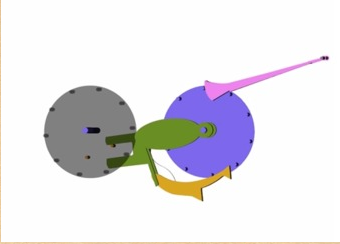
\includegraphics[scale=0.5]{../images/carry.png}
Carry Mechanism
\\
\\
 On the top side of the right wheel, we see a so-called stop-arm, that can turn around axis B, that is positioned on the left side of the right wheel. When the right wheel is turned clockwise, this arm is lifted by the passing pin. When the pin passes the arm, the arm falls down again and increases the count of the left wheel by 1. Thus performing the carry operation\cite{Article}.

Similarly, subtraction is performed by adding 10's complement of second number instead of the second number

\section{Original Design}
The pascaline in its original form is essentially a 3-D object,to simulate it in box2D we thought of showing it from side view.
\\
\\
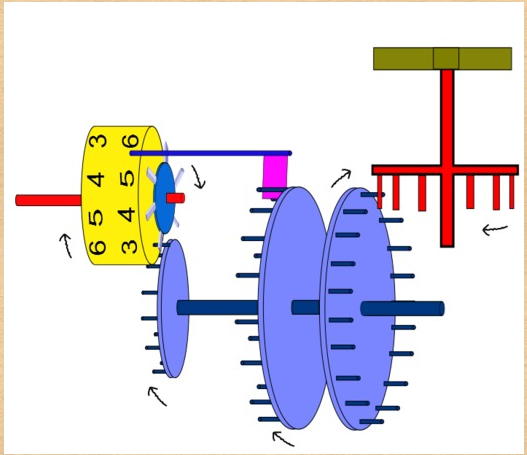
\includegraphics[scale=0.4]{../images/OriginalDesign.png}
Inkscape Design
\\
\\
So the blue circles with spokes would look like rectangle having spokes which are moving in SHM (simple harmonic motion).

\section{Final Design}
Our Initial approach of showing pascaline from side view resulted in circles with spokes looking like this -
\\
\\
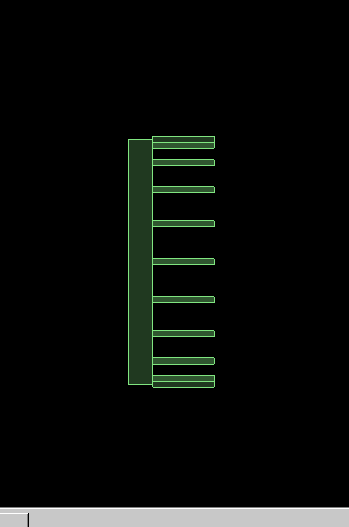
\includegraphics[scale=0.25]{../images/OriginalGear.png} 
Side view of original gear
\\
\\
This was not looking too nice so we decided to change the desgin    a bit.
To neatly show all the components we changed the plane of input dial and brought it in the same plane as others and replaced spoked circles with gears.
\\
\\
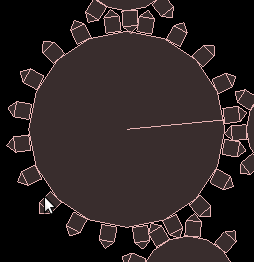
\includegraphics[scale=0.5]{../images/Gear.png} 
Final design of gear
\\
\\
Another change we made was that we changed the carry mechanism.In actual pascaline the weights of stop-arm and inertia of rotating wheels are carefully chosen so that on releasing stop-arm next digit increases only by one but we were not able to get actual data and hence desired result.

So we changed that by introducing another wheel having only 2 spokes which rotates by half the angle as input dial.So when input dial increases by 360 degrees this wheel rotates by half and increases next output wheel by one.

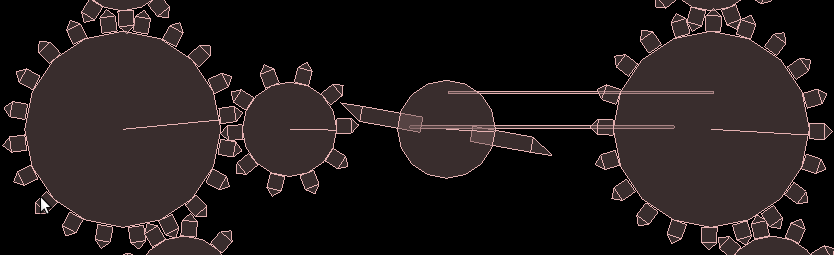
\includegraphics[scale=0.45]{../images/CarryMechanism.png} 
\\
Carry Mechanism
\\
\\
\textbf{Components of Simulation} -
\\
\\
\textbf{Gears} - gears are made by first taking a circle of appropriate radius and then adding rectangles to  it and then triangles on top of rectangles (this is done because gears with pentagonal spokes work better than ones with rectangular spokes).Density of gears differ from one another.Input dials have to rotate others , so they have been given higher density.Also the units digit part has to rotate the tens digit one therefore has higher density.
\\
\\
\textbf{Hinges} - Hinges are used to stop the gears from moving in opposite direction.This is made by adding two fixtures having a polygon shape two a high density body.
\\
\\
\textbf{Connectors} - Connectors are rectangular bars that makes the two spoked wheel rotate by same angle as the governer(bigger gear on units digit side).
These are made by using SetAsBox function  to give shape to fixture.
\\
\\
Some interseting things about final design-
\\
\\
To make the input dial moves gradually we rotated the input dials in the   step function 2 degrees at a time.
\\
To rotate a gear we have used two types of mechanisms - 
one causes  the gears to move by same angle, this is done by adding bars between gears.   
other that moves the gears by same angular displacement,this is done by interlocking the teeths of gears.
\\
\\
\\
\\
\\
\\
Our final design looks like this -
\\
\\
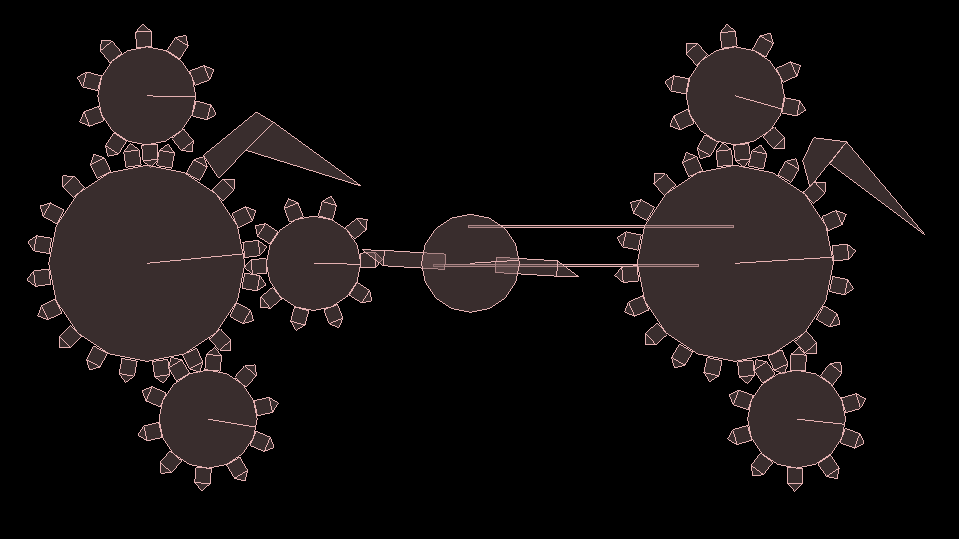
\includegraphics[scale=0.4]{../images/FinalDesign.png}
Final structure of simulation
\\
\\
\section{Analysis of plots}
We have plotted the graphs for data set of 1000 iterations and 5 re-runs.
The observed plots are quite similar to ones we obtained from lab09.

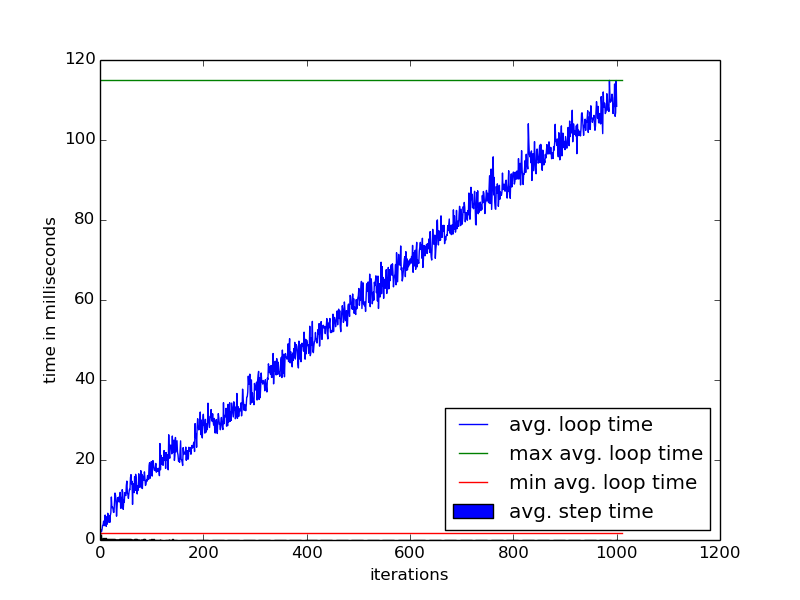
\includegraphics[width=\textwidth,height = 7.5cm]{../images/g08_plot01.png}
Plot 1
\\

In Plot 1 we observe that average step time is quite high in the starting
and it reduces quite fast, but as the number of iterations increases, the rate at which it decreases becomes low and the value starts to stabilize. 
It can be explained as the number of collisions in the starting is quite high and it takes time to resolve these. Total loop time increases approximately linearly with number of iterations (neglecting small variations). This was also expected since after some iterations, value of step time becomes approximately constant, and  loop time is approximately sum of step time, thus it comes out to be somewhat linear. 

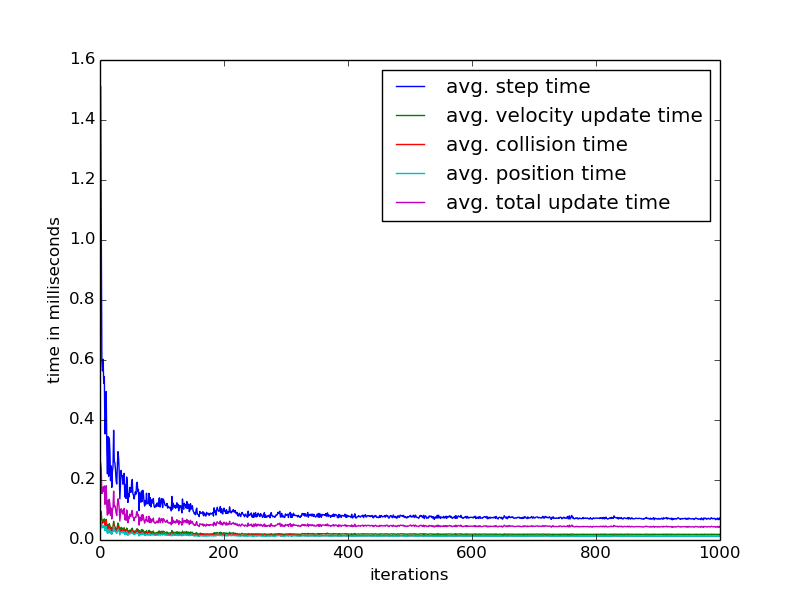
\includegraphics[width=\textwidth,height = 6.5cm]{../images/g08_plot02.png}
Plot 2
\\
	
In Plot 2 we see the same behaviour of step time as in Plot 1, but the interesting thing here is that bulk of the update time is constituted by velocity update i.e solveVelocity function. This function takes up most of the time. We also see that step time is higher than update time but has almost same shape. This was also expected since all the update functions i.e Velocity, Position and Collision functions are part of step function. 

From this plot we observe a small peak at iteration number 200 which gradually reduces ,this is because around this point our two spoked circle comes in contact with other circle and causes lots of contacts and thus more calculations.It decreases  as later number of iterations increases while calculations required are lesser than at iteration 200.


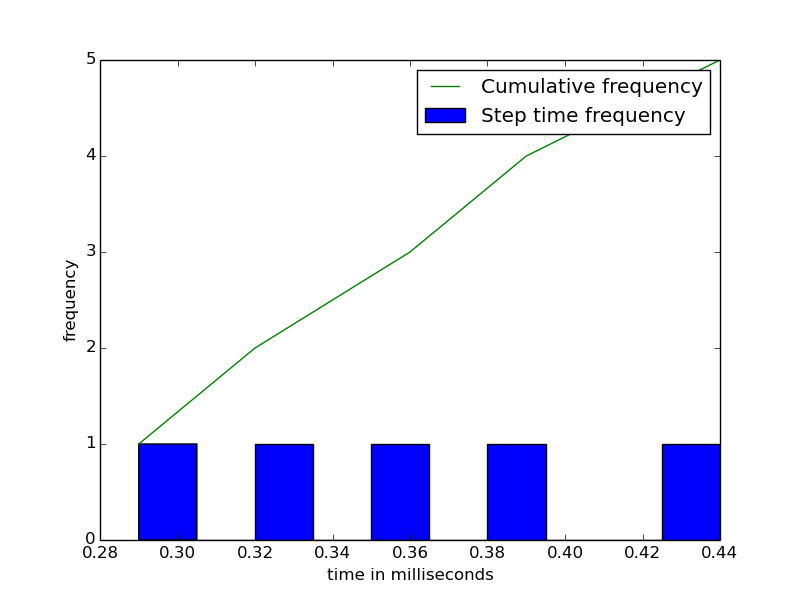
\includegraphics[width=\textwidth,height = 6.5cm]{../images/g08_plot04.png}
Plot 4
\\

In Plot 4, if we assume the heights of bars are mass and find the center of
mass we will get average step time for that iteration. 

\section{Profiling}
Profiling is a form of dynamic program analysis that measures, the space and time complexity of a program, the usage of particular instructions, the frequency and duration of function calls, etc. The most common use of profiling information is to aid program optimization. Profiling is achieved by instrumenting either the program source code or its binary executable form using a tool called a profiler. Both gprof and perf are common performance analysis tools which can be used for profiling. We used perf as it was generating more detailed call graphs using the command which generates the data file for the debug build. To ensure that profiling can occur we must add the -pg option when compiling so that information relevant for profiling is generated during compilation.

\subsection{Debug Build}
The Debug Build was made by adding the option \textbf{-DCMAKE-BUILD-TYPE=Debug} to the cmake command when installing Box2D. The program was run for 10000 iterations.
\\
\begin{center}
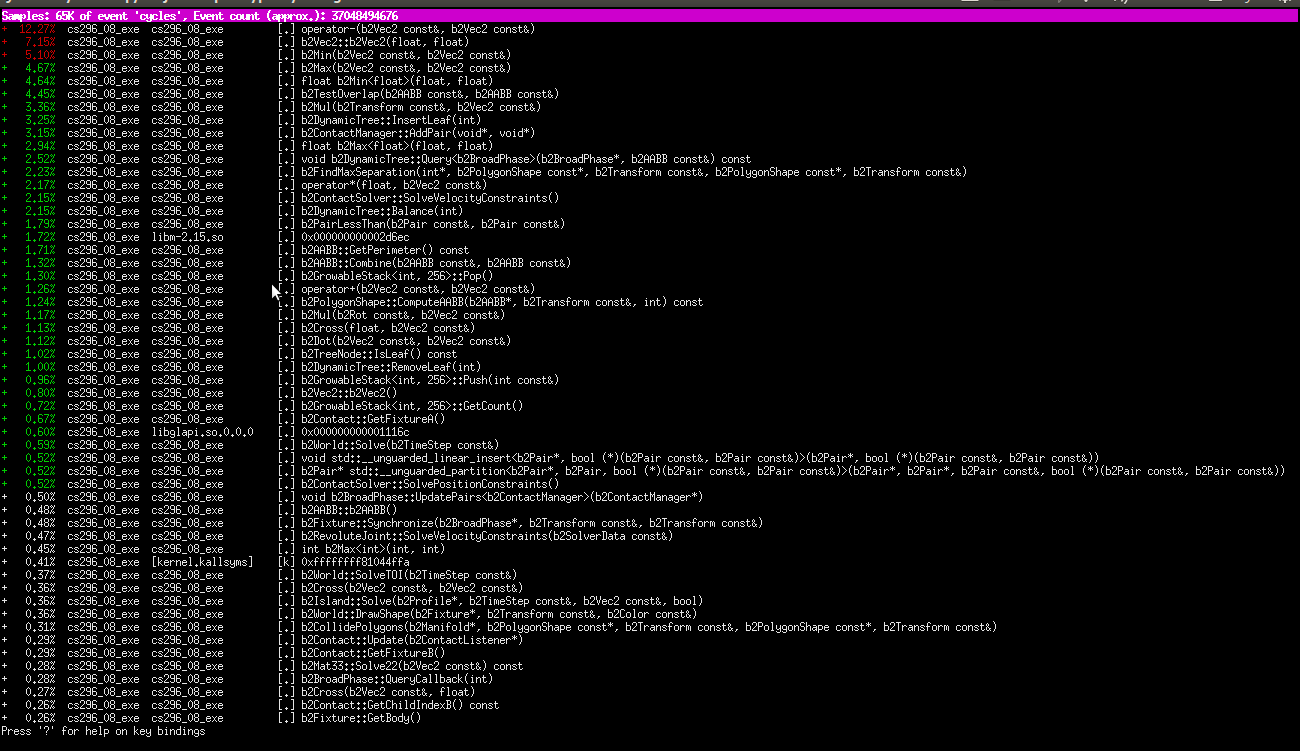
\includegraphics[width=15cm,height = 6cm]{../images/debug.png}
The profile for debug build.
\\
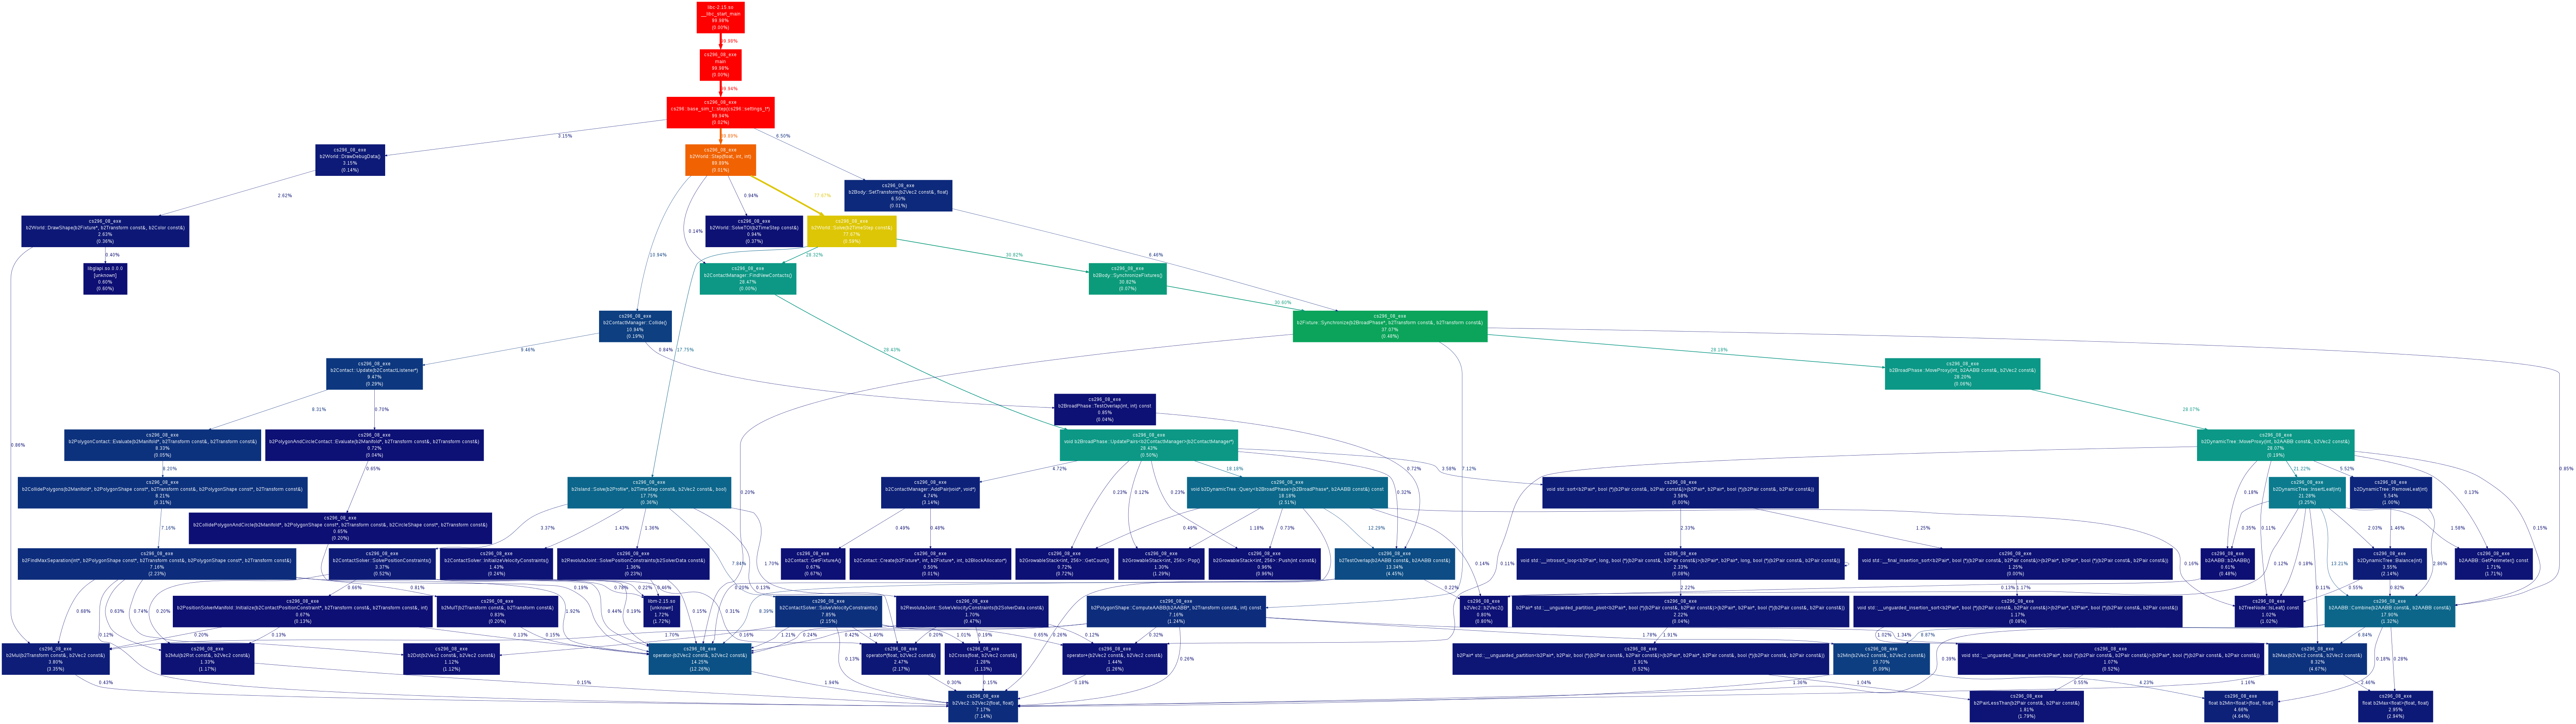
\includegraphics[width=15cm,height = 6cm]{../images/debug_call_graph.png}
The call graph for debug build.
\\
\end{center}

\subsection{Release Build}
The Release Build was made by adding the option \textbf{ -DCMAKE-BUILD-TYPE=Release} to the cmake command when installing Box2D. The flags -O2 and -O3 were also added to the cppflags while compiling the program using release build. These flags are explained later. The program was run for 10000 iterations.

\begin{center}
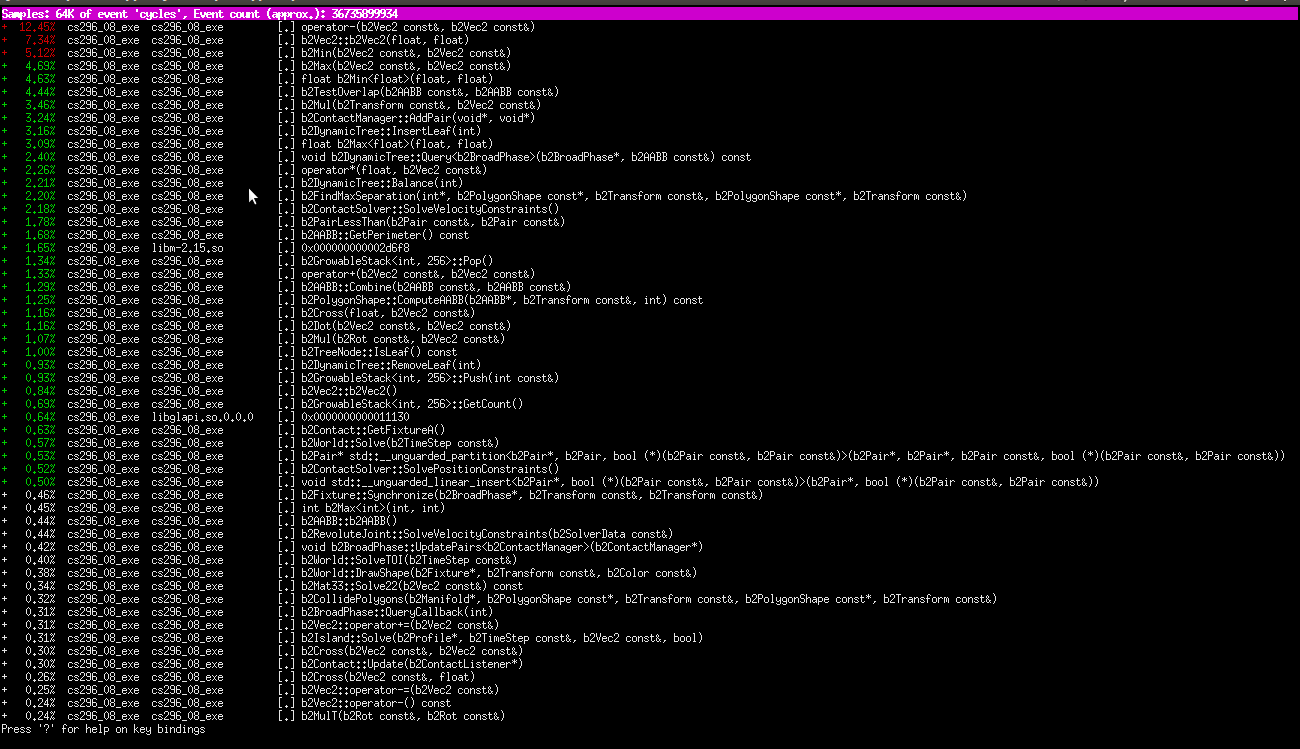
\includegraphics[width=15cm,height = 6cm]{../images/release.png}
The profile for release build.
\\
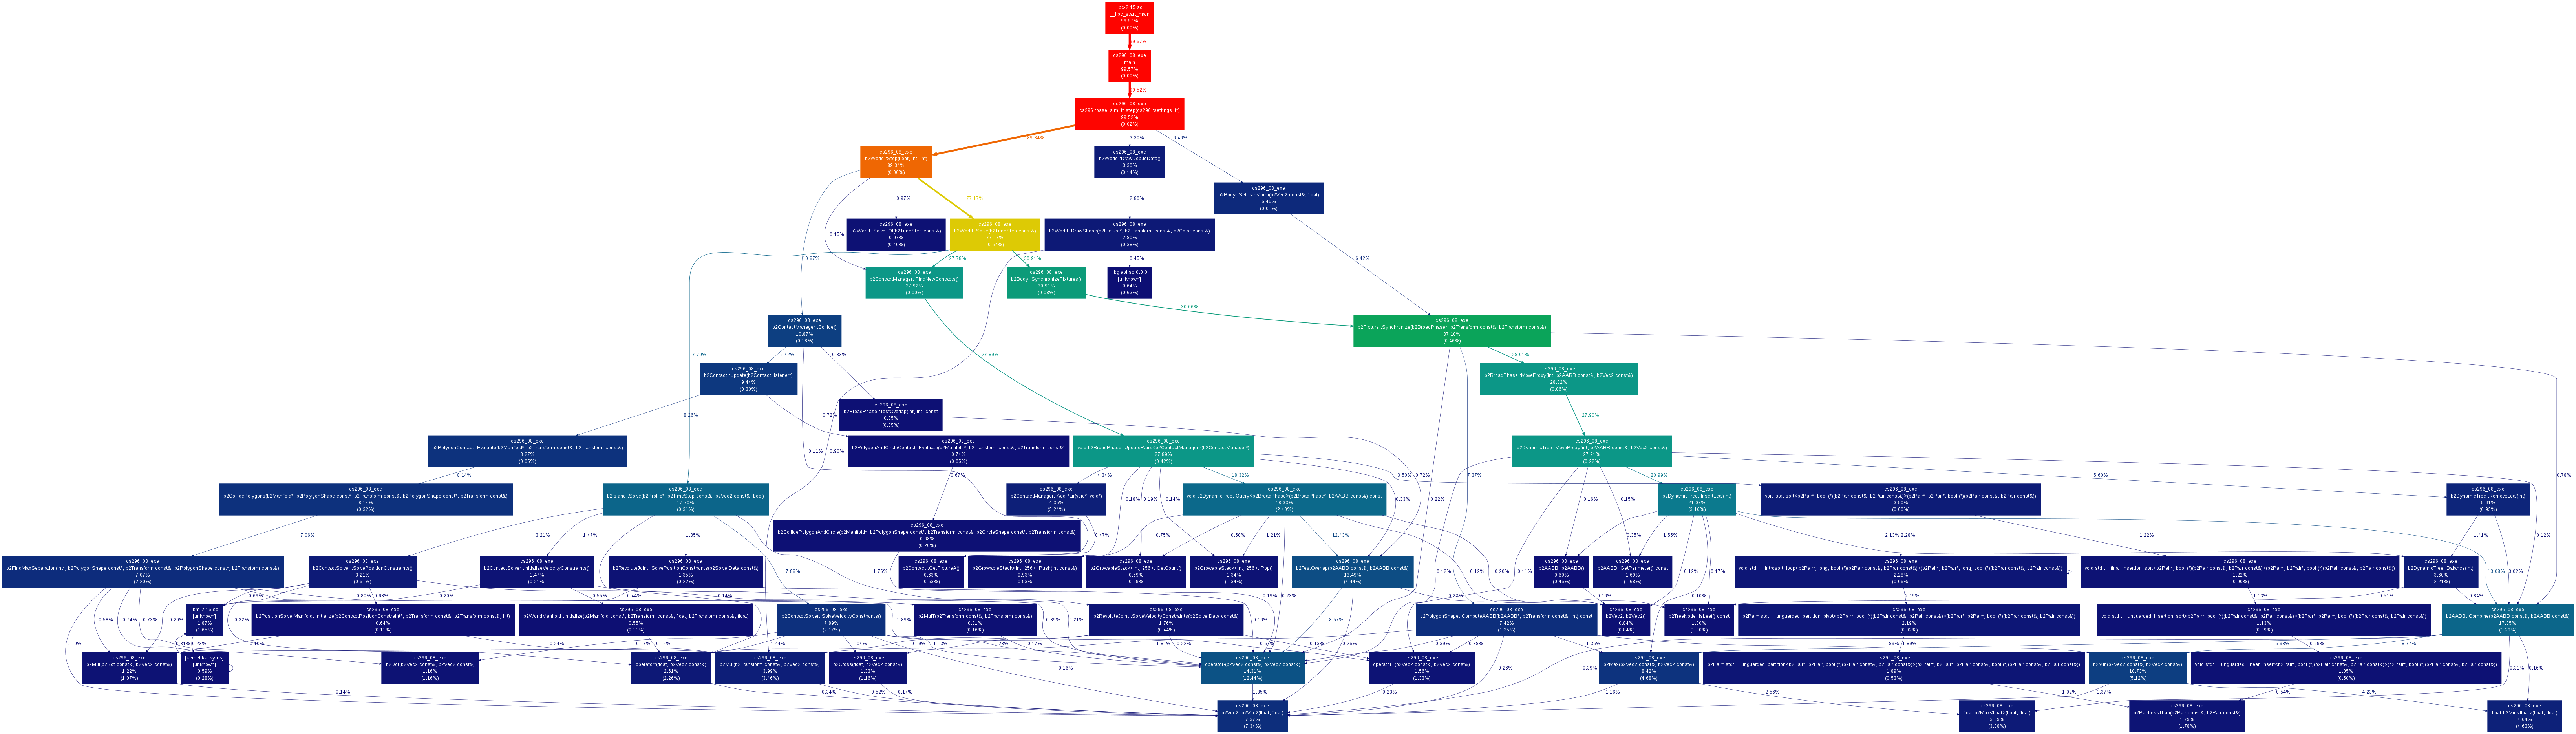
\includegraphics[width=15cm,height = 6cm]{../images/release_call_graph.png}
The call graph for release build.
\\
\end{center}

\subsection{Inference}
After optimization it is clear from the profiles that the same processes have fewer occurences in the release build. Also the overhead of the Box2D functions is generally lesser in the release build which whows that they have more optimization while the overhead of the gui functions such as those used for mesa increase which shows a relatively lesser amount of optimization for them. Functions such as b2ContactSolver which have higher number of occurences in the debug build and a large change when compared to the release build are the functions which require optimization the most (functions which show little change do not change running time much after optimization no matter how much overhead they have).

\subsection{Difference between Debug and Release build}
The major difference between the Debug and Release build is clear by the name. The Release build is made assuming that the user only uses the application for final use and is not meant for debugging. Hence the program does not release debugging-relevant information. This is also clear from the call-graph of the release build which contains various unresolved functions given in the form of hex pointers. Also, various modes of optimization such as inlining and loop-unrolling which decrease the running time of the program are not allowed in Debug mode. Hence, the debug build for the same program and the same number of iterations will have many more function calls and take more time than the corresponding release build.

\subsection{Optimization - O2 and O3}
O2 and O3 are both optimization options for the gcc command which result in various optimization techniques being used while compiling the code such as inlining and loop-unrolling. These options increase the performance of the program at the cost of higher compilation time. O3 is a more powerful optimization as compared to O2 but might result in tradeoff between space and time.

\bibliographystyle{plain}
\bibliography{bibliographies}
\end{document}